\begin{figure}[t]
    \centering
    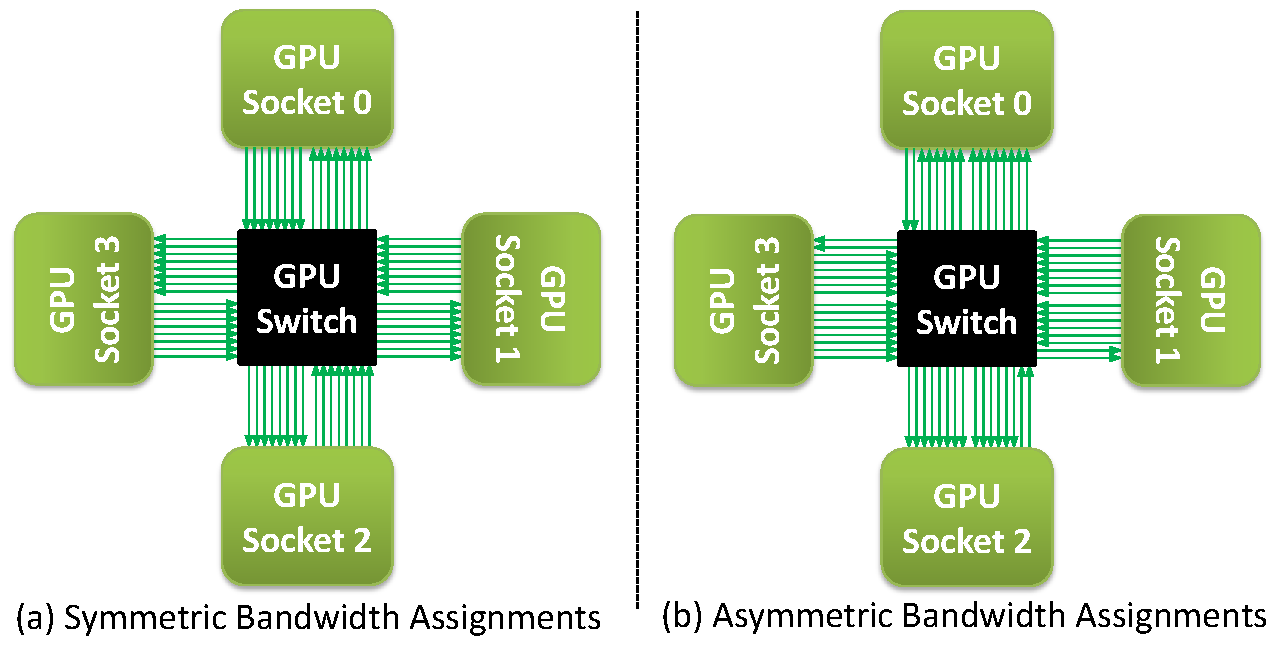
\includegraphics[width=1.0\columnwidth]{figures/tms_links.pdf}
    \caption{Multi-socket GPU systems with symmetric and assymeteric capacity assignments.}
    \label{fig:symmetric_assymetric}
\end{figure}

\begin{figure}[t]
    \centering
    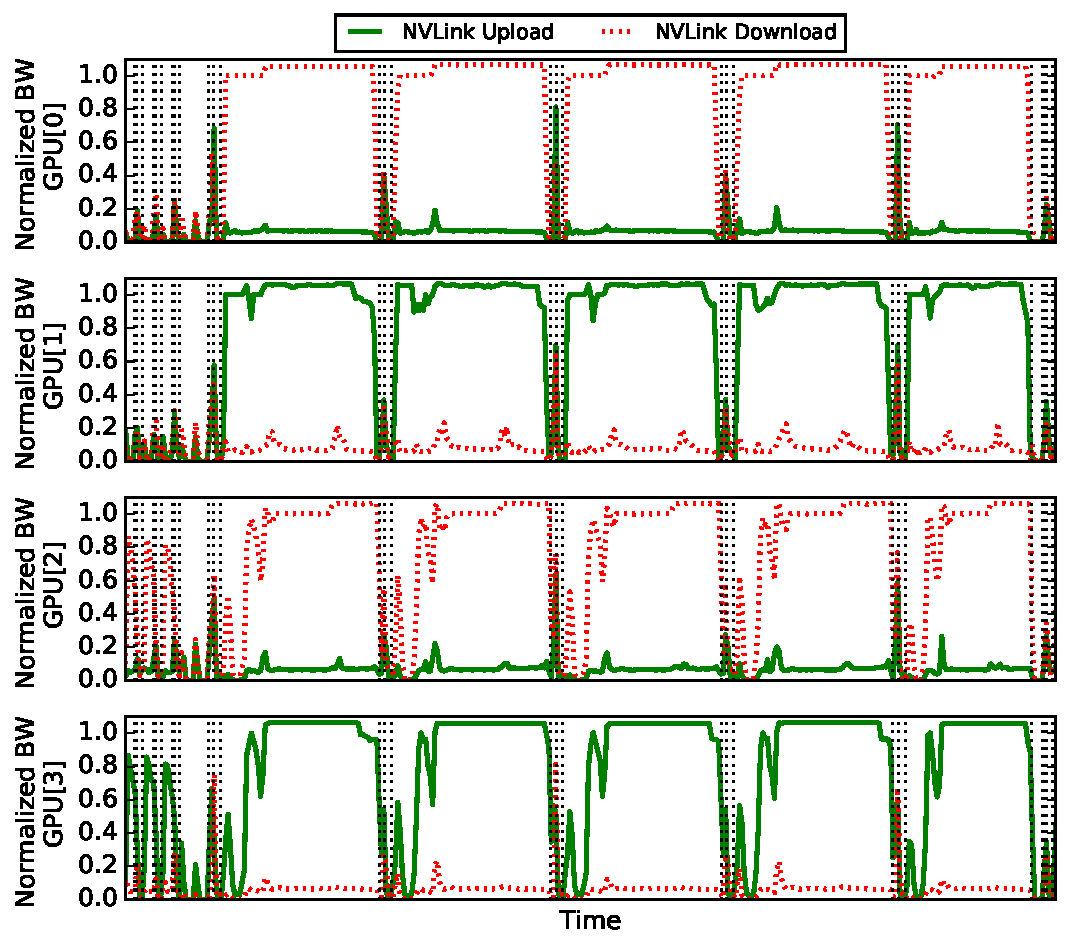
\includegraphics[width=1.0\columnwidth]{figures/bw_profile_HPGMG_UVM_base.pdf}
    \caption{Normalized NVLink bandwidth profile for \texttt{HPC-HPGMG-UVM} showing example of asymmetric 
    link utilization between GPUs and within a GPU depending on kernel and application phasing.}
    \label{fig:link-motivation}
\end{figure}

\section{Asymmetric Links for TMS-GPUs}
\label{interconnect}

Figure~\ref{fig:symmetric_assymetric}(a) shows a generic multi-socket system
with symmetric bandwidth assignments at each inter-socket communication link.
Static link capacity assignment at design time is very common and has multiple
advantages. For example, in such case only one type of I/O circuitry (egress
drivers or ingress receivers) along with only one type of control logic need to
be implemented at each on-chip interface. Moreover, multi-socket switches
result in simpler designs that support a statically provisioned worst-case
bandwidth scenario. On the other hand, multi-socket link bandwidth has a very
important impact on overall system performance. For the applications which saturate links between sockets, doubling NVLink capacity potentially achieves a 2$\times$ speedup.
%As shown in Figure~\ref{fig:switchtime}, where doubling NVLink capacity from 128GB/s to 256GB/s reached 1.5x average speedup reaching a 2x speedup for many applications. 
As I/O bandwidth is a very limited and expensive resource, this
result motivates us to look for alternatives that keep wire and I/O resources
at very high utilization. 

We note that the typically employed symmetric link
capacity assignments may result in lower overall utilization of the link wires
in many cases. Moreover, in case of TMS-GPU systems, we do observe that there
are applications in which some GPUs have a very different utilization of its
egress and ingress channels in different phases of execution.
Figure~\ref{fig:link-motivation} shows dynamic link utilization for a snapshot
of \texttt{HPC-HPGMG-UVM} application running on our baseline 4 GPUs TMS-GPU
system. Vertical dotted black lines represent the beginning kernel calls that
are split across 4 sockets as explained in Section~\ref{background}. We can see
that few initial small kernels have a negligible interconnect
utilization on all links. However, for the the upcoming larger kernels at the
figure, GPU0 and GPU2 fully saturate their ingress links, while GPU1 and GPU3
fully saturate their egress links. At the same time GPU0 and GPU2 pair,
and GPU1 and GPU3 pair barely use their egress or ingress links accordingly.

\begin{figure*}[tp]
    \centering
    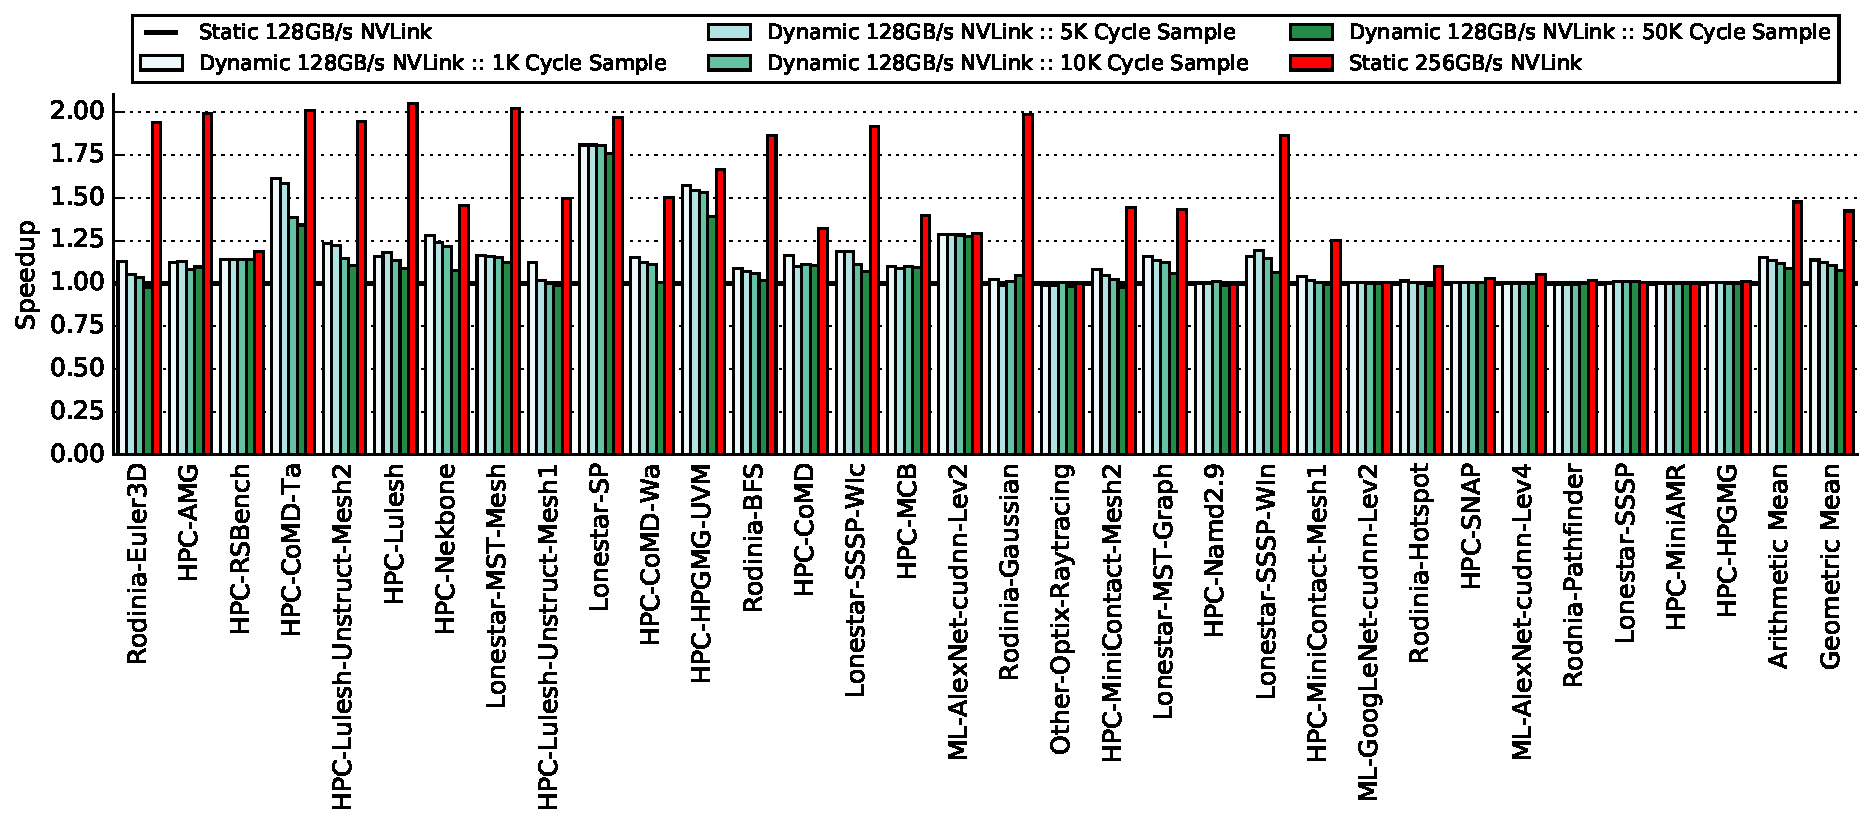
\includegraphics[width=1.0\textwidth]{figures/plot_nvlink_sample_time.pdf}
    \caption{Relative speedup of the dynamic NVlink adaptivity with respect to
	the baseline architecture by varying sample time and assuming switch time of
	100 cycles. In red, relative speedup achievable by doubling the bandwidth.}
    \label{fig:sampletime}
\end{figure*}

Motivated by these findings, we propose to dynamically control multi-socket
link bandwidth assignments in each direction on a per-GPU basis resulting in
dynamically asymmetric link capacity assignments, as shown in
Figure~\ref{fig:symmetric_assymetric}(b). Such dynamic and asymmetric link
capacity distribution is expected to yield higher wire utilization and
essentially higher effective bandwidth and performance for a given set of I/O
resources. This mechanism is somewhat similar to DRAM interface for example,
where the same set of wires is used for both read and write directions
interchangeably, and link direction is reversed based on a dynamic state of the
system~\textbf{need some citation here}. 

For basic link configuration we assume and model point-to-point
links with multiple lanes each, similarly to NVLink
sub-links~\cite{pascal-tesla-wp}.  In such link, 8 lanes with 8GB/s capacity
per lane results in an aggregate bandwidth of 64GB/s in each direction. We
propose an adaptive asymmetric scheme that works as following. For each link
in the system, at kernel launch we start with symmetric link assignments with 8
lanes per direction. Then, we propose to periodically sample the saturation
status of each link. If the lanes in one direction are not saturated, while the
lanes in the opposite direction are 99\% saturated, we reverse the direction of
one of the unsaturated lanes. Periodically repeating and sampling the lanes
status, we stop either when equilibrium is reached, or alternatively all the 
lanes but one have been reversed (we always keep a minimum bandwidth of 8GB/s 
in each direction).  
%We have a threshold of 
%1GB/sec to prevent switching for minimum variations in traffic shape.  
% EVGENY - I dint get it\ldots if you belive its importnat rephrase.  
There are two important factors that characterize the behaviour above (i) 
\texttt{SampleTime}: the frequency at which the scheme samples for a possible 
reconfiguration and (ii) \texttt{SwitchTime}: the cost of switching the 
direction of a lane. Switching period is comprised of the time it takes to 
drain all the pending packets in a given direction, and the time it takes to 
physically reconfigure the lane to start transmitting in the opposite 
direction. 
------  Evgeny : still need to add what are teh disadvnatages of assymetric
(double IO interfaces and switching complexity)



\subsection{Results}
Figure~\ref{fig:sampletime} shows the performance improvement, with respect 
to our baseline architecture by exploring different values of the 
\texttt{SampleTime} and assuming a \texttt{SwitchTime} of 100 cycles as 
reported in~\cite{REALLY_NEED_REF_HERE}. Also, Figure~\ref{fig:sampletime} 
gives an upper-bound performance when doubling the available interconnect 
bandwidth to 256GB/s (128GB/s per direction). For the benchmarks on the right 
side, where the baseline TMS-GPU performs close to 4$\times$ larger single 
GPU, increasing the inter-socket bandwidth does not improve performance 
significantly. Contiguous CTA scheduling and first-touch memory placement 
preserves good data locality in those cases, so that both ingress and egress 
links are underutilized. On the left side, we can see that for some 
applications, 2$\times$ NVLink bandwidth translates to 2$\times$ speedup, 
while dynamic lane switching achieves up to 80\% performance improvement 
(\texttt{Lonestar-SP}). On average, double the interconnect bandwidth gives 
50\% while our dynamic solution achieves 15\% improvements. We can also see 
that the sampling frequency plays a critical role and a too large sample time 
doesn't capture application dynamics resulting in smaller improvements. We 
find 5K cycles to be a reasonable sampling period able to achieve good 
results and never degrade performance. 

Another important parameter is switching period needed to turn around a 
single lane direction. Our results point that higher \texttt{SwitchTime} 
values, like 200 and 500 cycles, only degrade the average performance by less 
than 2\% compared to 100 cycle switching period. We observe the maximum 
slowdown of 25\% in case of \texttt{HPC-CoMD-Ta} and \texttt{HPC-CoMD-Wa} 
when switch time reaches 500 cycles. At the same time, faster lane switch (10 
cycles) does not improve the performance compared to 100 cycles. Thus from 
now, we define our adaptive link assignment policy which samples saturation 
status on every 5K cycles and eventually turn link direction with 100 cycles 
penalty. 

%In Figure~\ref{fig:switchtime} we used 5K cycles sample time to
%explore values of ``switch\_time'' from 10 cycles to 500 cycles.
%We found that a faster switch does not produce better results than 100 cycles
%but that in few applications a long (500 cycles) switch time results 25\% 
%less performance with respect to 100 cycles (``HPC-CoMD-Ta'' and 
%``HPC-CoMD-Wa'').

% Graph 0: We need a stacked-bar graph that shows what’s the percentage of total 
% exe time spent in configs where: both directions are saturated (no room for 
% improvement), only one direction is saturated (here we can improve), none is 
% saturated (we don’t care for this). Do we want to show this as aggregate number 
% of per-GPU?
% We explain the algorithm how and when we increment and decrement the number of 
% sub-channels per direction. Two important parameters: link switch time and 
% sample time.

% Graph 1: baseline is 1x NVLink, upper bound is 2x NVLink, link switch time is 
% 100 cycles, we show the speedup for different sample time values (1K, 2K, 5K, 
% 10K, 100K cycles). Finner measurements are better.

% Graph 2a: baseline is 1x NVLink, upper bound is 2x NVLink, sample\_time is 1K. 
% We swipe through link\_switch\_time (10, 100, 200, 500 cycles). Here, link 
% switch time is important, we want it to be low.

% Graph 2b: the same, but sample\_time is 100K. Here, we do not care about link 
% switch time. The point where it starts to matter is 5K (or 2K) cycles and below. 
% From now on, we assume 100 cycles for link switch time and 5K (or 2K) cycles for 
% sampling period.


% DO NOT REMOVE, we can use this to compute POWER later
%from http://teams.nvidia.com/sites/Corporate/ntech/SiteAssets/downloads/2014/NTECH2014_SlideDecks%20(presented)/7.1_Osborn.pptx
%Power: 8 lanes (TX + RX) at 25GT/s ~= 1.5W
%Area: 8 Lane PHY (8 TX + 8 RX + PLL) ~= 3.3mm^2
%Physical Data: .5pJ/b transferred


%\begin{figure*}[tp]
%   \centering
%   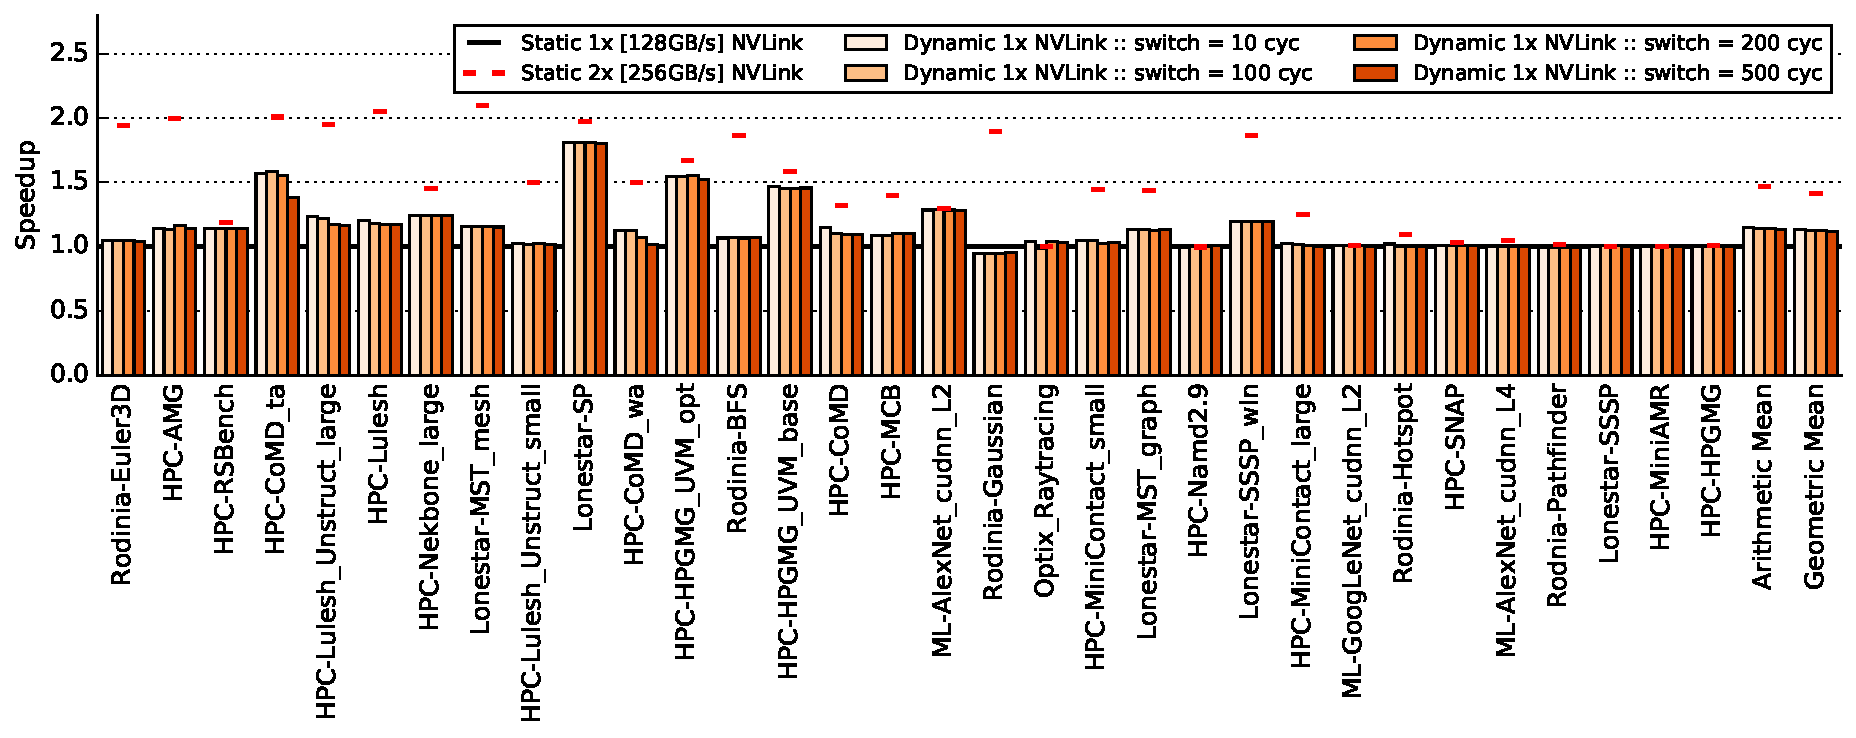
\includegraphics[width=1.0\textwidth]{figures/plot_nvlink_switch_time_sample_time5000.pdf}
%   \caption{Relative speedup of the dynamic NVlink adaptivity with respect to
%	the baseline architecture varying switch time for a fixed sample time
%of 5k cycles. In red, relative speedup achievable by doubling the bandwidth.}
%    \label{fig:switchtime}
%\end{figure*}
